\documentclass[11pt,preprint, authoryear]{elsarticle}

\usepackage{lmodern}
%%%% My spacing
\usepackage{setspace}
\setstretch{1.2}
\DeclareMathSizes{12}{14}{10}{10}

% Wrap around which gives all figures included the [H] command, or places it "here". This can be tedious to code in Rmarkdown.
\usepackage{float}
\let\origfigure\figure
\let\endorigfigure\endfigure
\renewenvironment{figure}[1][2] {
    \expandafter\origfigure\expandafter[H]
} {
    \endorigfigure
}

\let\origtable\table
\let\endorigtable\endtable
\renewenvironment{table}[1][2] {
    \expandafter\origtable\expandafter[H]
} {
    \endorigtable
}


\usepackage{ifxetex,ifluatex}
\usepackage{fixltx2e} % provides \textsubscript
\ifnum 0\ifxetex 1\fi\ifluatex 1\fi=0 % if pdftex
  \usepackage[T1]{fontenc}
  \usepackage[utf8]{inputenc}
\else % if luatex or xelatex
  \ifxetex
    \usepackage{mathspec}
    \usepackage{xltxtra,xunicode}
  \else
    \usepackage{fontspec}
  \fi
  \defaultfontfeatures{Mapping=tex-text,Scale=MatchLowercase}
  \newcommand{\euro}{€}
\fi

\usepackage{amssymb, amsmath, amsthm, amsfonts}

\def\bibsection{\section*{References}} %%% Make "References" appear before bibliography


\usepackage[round]{natbib}

\usepackage{longtable}
\usepackage[margin=2.3cm,bottom=2cm,top=2.5cm, includefoot]{geometry}
\usepackage{fancyhdr}
\usepackage[bottom, hang, flushmargin]{footmisc}
\usepackage{graphicx}
\numberwithin{equation}{section}
\numberwithin{figure}{section}
\numberwithin{table}{section}
\setlength{\parindent}{0cm}
\setlength{\parskip}{1.3ex plus 0.5ex minus 0.3ex}
\usepackage{textcomp}
\renewcommand{\headrulewidth}{0.2pt}
\renewcommand{\footrulewidth}{0.3pt}

\usepackage{array}
\newcolumntype{x}[1]{>{\centering\arraybackslash\hspace{0pt}}p{#1}}

%%%%  Remove the "preprint submitted to" part. Don't worry about this either, it just looks better without it:
\makeatletter
\def\ps@pprintTitle{%
  \let\@oddhead\@empty
  \let\@evenhead\@empty
  \let\@oddfoot\@empty
  \let\@evenfoot\@oddfoot
}
\makeatother

 \def\tightlist{} % This allows for subbullets!

\usepackage{hyperref}
\hypersetup{breaklinks=true,
            bookmarks=true,
            colorlinks=true,
            citecolor=blue,
            urlcolor=blue,
            linkcolor=blue,
            pdfborder={0 0 0}}


% The following packages allow huxtable to work:
\usepackage{siunitx}
\usepackage{multirow}
\usepackage{hhline}
\usepackage{calc}
\usepackage{tabularx}
\usepackage{booktabs}
\usepackage{caption}


\newenvironment{columns}[1][]{}{}

\newenvironment{column}[1]{\begin{minipage}{#1}\ignorespaces}{%
\end{minipage}
\ifhmode\unskip\fi
\aftergroup\useignorespacesandallpars}

\def\useignorespacesandallpars#1\ignorespaces\fi{%
#1\fi\ignorespacesandallpars}

\makeatletter
\def\ignorespacesandallpars{%
  \@ifnextchar\par
    {\expandafter\ignorespacesandallpars\@gobble}%
    {}%
}
\makeatother

\newenvironment{CSLReferences}[2]{%
}

\urlstyle{same}  % don't use monospace font for urls
\setlength{\parindent}{0pt}
\setlength{\parskip}{6pt plus 2pt minus 1pt}
\setlength{\emergencystretch}{3em}  % prevent overfull lines
\setcounter{secnumdepth}{5}

%%% Use protect on footnotes to avoid problems with footnotes in titles
\let\rmarkdownfootnote\footnote%
\def\footnote{\protect\rmarkdownfootnote}
\IfFileExists{upquote.sty}{\usepackage{upquote}}{}

%%% Include extra packages specified by user

%%% Hard setting column skips for reports - this ensures greater consistency and control over the length settings in the document.
%% page layout
%% paragraphs
\setlength{\baselineskip}{12pt plus 0pt minus 0pt}
\setlength{\parskip}{12pt plus 0pt minus 0pt}
\setlength{\parindent}{0pt plus 0pt minus 0pt}
%% floats
\setlength{\floatsep}{12pt plus 0 pt minus 0pt}
\setlength{\textfloatsep}{20pt plus 0pt minus 0pt}
\setlength{\intextsep}{14pt plus 0pt minus 0pt}
\setlength{\dbltextfloatsep}{20pt plus 0pt minus 0pt}
\setlength{\dblfloatsep}{14pt plus 0pt minus 0pt}
%% maths
\setlength{\abovedisplayskip}{12pt plus 0pt minus 0pt}
\setlength{\belowdisplayskip}{12pt plus 0pt minus 0pt}
%% lists
\setlength{\topsep}{10pt plus 0pt minus 0pt}
\setlength{\partopsep}{3pt plus 0pt minus 0pt}
\setlength{\itemsep}{5pt plus 0pt minus 0pt}
\setlength{\labelsep}{8mm plus 0mm minus 0mm}
\setlength{\parsep}{\the\parskip}
\setlength{\listparindent}{\the\parindent}
%% verbatim
\setlength{\fboxsep}{5pt plus 0pt minus 0pt}



\begin{document}



\begin{frontmatter}  %

\title{22581340\_Music}

% Set to FALSE if wanting to remove title (for submission)




\author[Add1]{Gabriella Neilon}
\ead{22581340@sun.ac.za}





\address[Add1]{Stellenbosch University}

\cortext[cor]{Corresponding author: Gabriella Neilon}

\begin{abstract}
\small{
This report delves into the aspects of popularity, style, and emotion
found within the studio albums of Coldplay and Metallica.
}
\end{abstract}

\vspace{1cm}





\vspace{0.5cm}

\end{frontmatter}

\setcounter{footnote}{0}



%________________________
% Header and Footers
%%%%%%%%%%%%%%%%%%%%%%%%%%%%%%%%%
\pagestyle{fancy}
\chead{}
\rhead{}
\lfoot{}
\rfoot{\footnotesize Page \thepage}
\lhead{}
%\rfoot{\footnotesize Page \thepage } % "e.g. Page 2"
\cfoot{}

%\setlength\headheight{30pt}
%%%%%%%%%%%%%%%%%%%%%%%%%%%%%%%%%
%________________________

\headsep 35pt % So that header does not go over title




\hypertarget{introduction}{%
\section{\texorpdfstring{Introduction
\label{Introduction}}{Introduction }}\label{introduction}}

In this report, I delve into the characteristics of two iconic bands,
Coldplay and Metallica, exploring their studio albums in terms of
popularity, style, and emotion. I analyse various factors such as
acousticness, danceability, energy, instrumentalness, loudness,
speechiness, valence, and tempo to gain insights into the unique
attributes of their music. Additionally, we examine the emotions evoked
by their albums, focusing on happiness and sadness as key emotional
indicators. By delving into these aspects, we aim to uncover the
distinct features that define the music of Coldplay and Metallica,
providing a deeper understanding of their artistic expressions.

\hypertarget{part-a}{%
\section{Part A}\label{part-a}}

In this section I explore the popularity per album of each band.

\hypertarget{coldplay}{%
\subsection{Coldplay}\label{coldplay}}

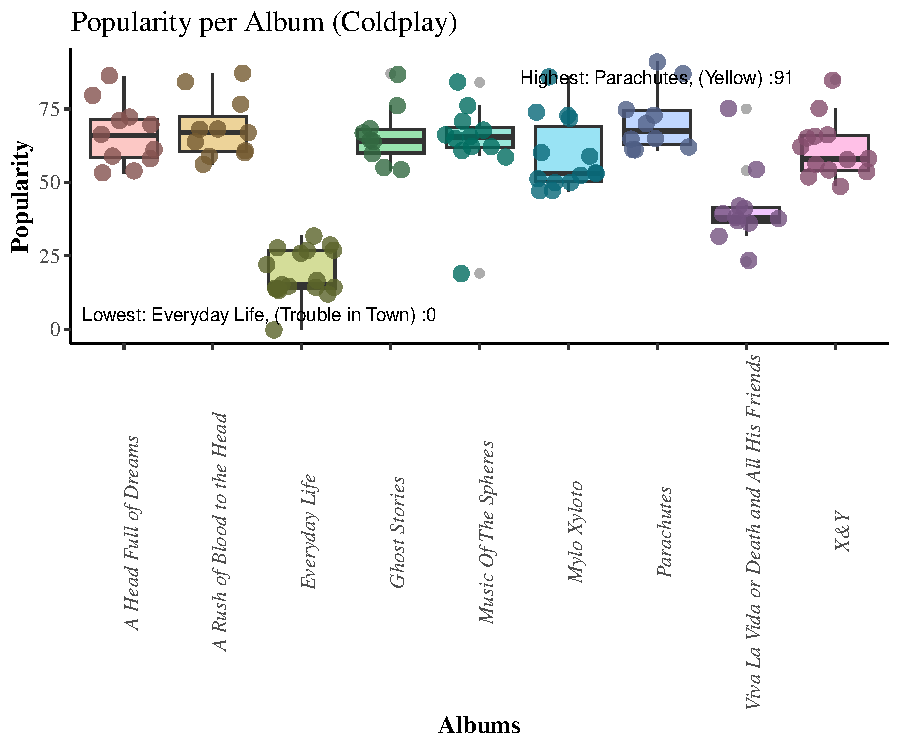
\includegraphics{Question3_files/figure-latex/unnamed-chunk-1-1.pdf}

This graph shows that the most popular album of Coldplay is
``Parachutes'', with the most favoured song ``Yellow''.

\hypertarget{metallica}{%
\subsection{Metallica}\label{metallica}}

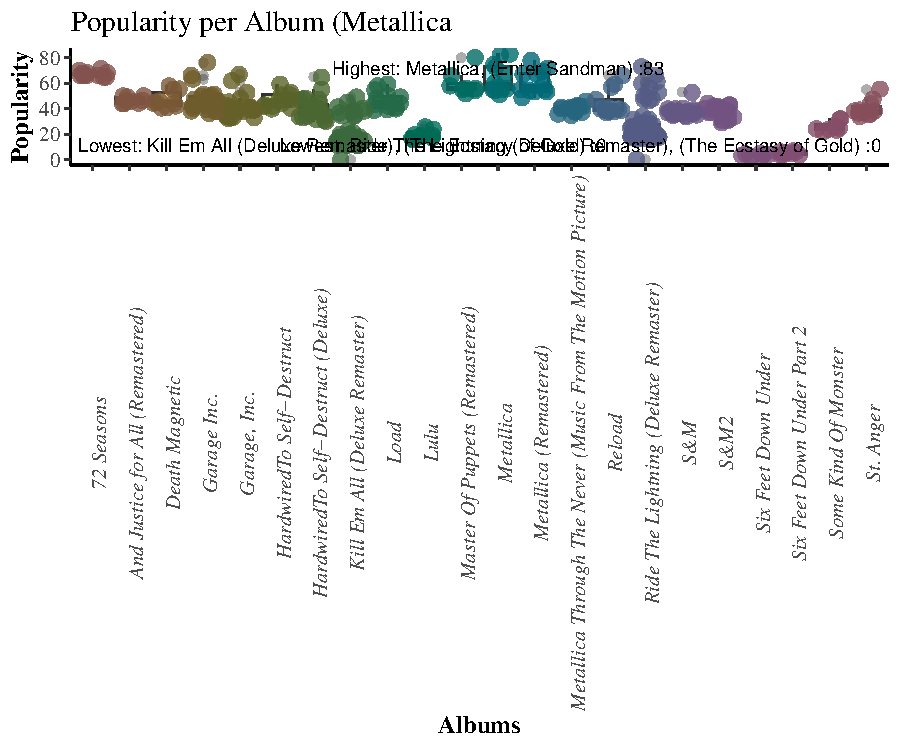
\includegraphics{Question3_files/figure-latex/unnamed-chunk-2-1.pdf}
This graph shows that the most popular album of Metallica is
``Metallica'', with the most favoured song ``Enter Sandman''.

Based on popularity, Coldplay is favoured over Metallica.

\hypertarget{part-b}{%
\section{Part B}\label{part-b}}

In this section I explore the style of the bands' styles across
different albums.

\hypertarget{coldplay-1}{%
\subsection{Coldplay}\label{coldplay-1}}

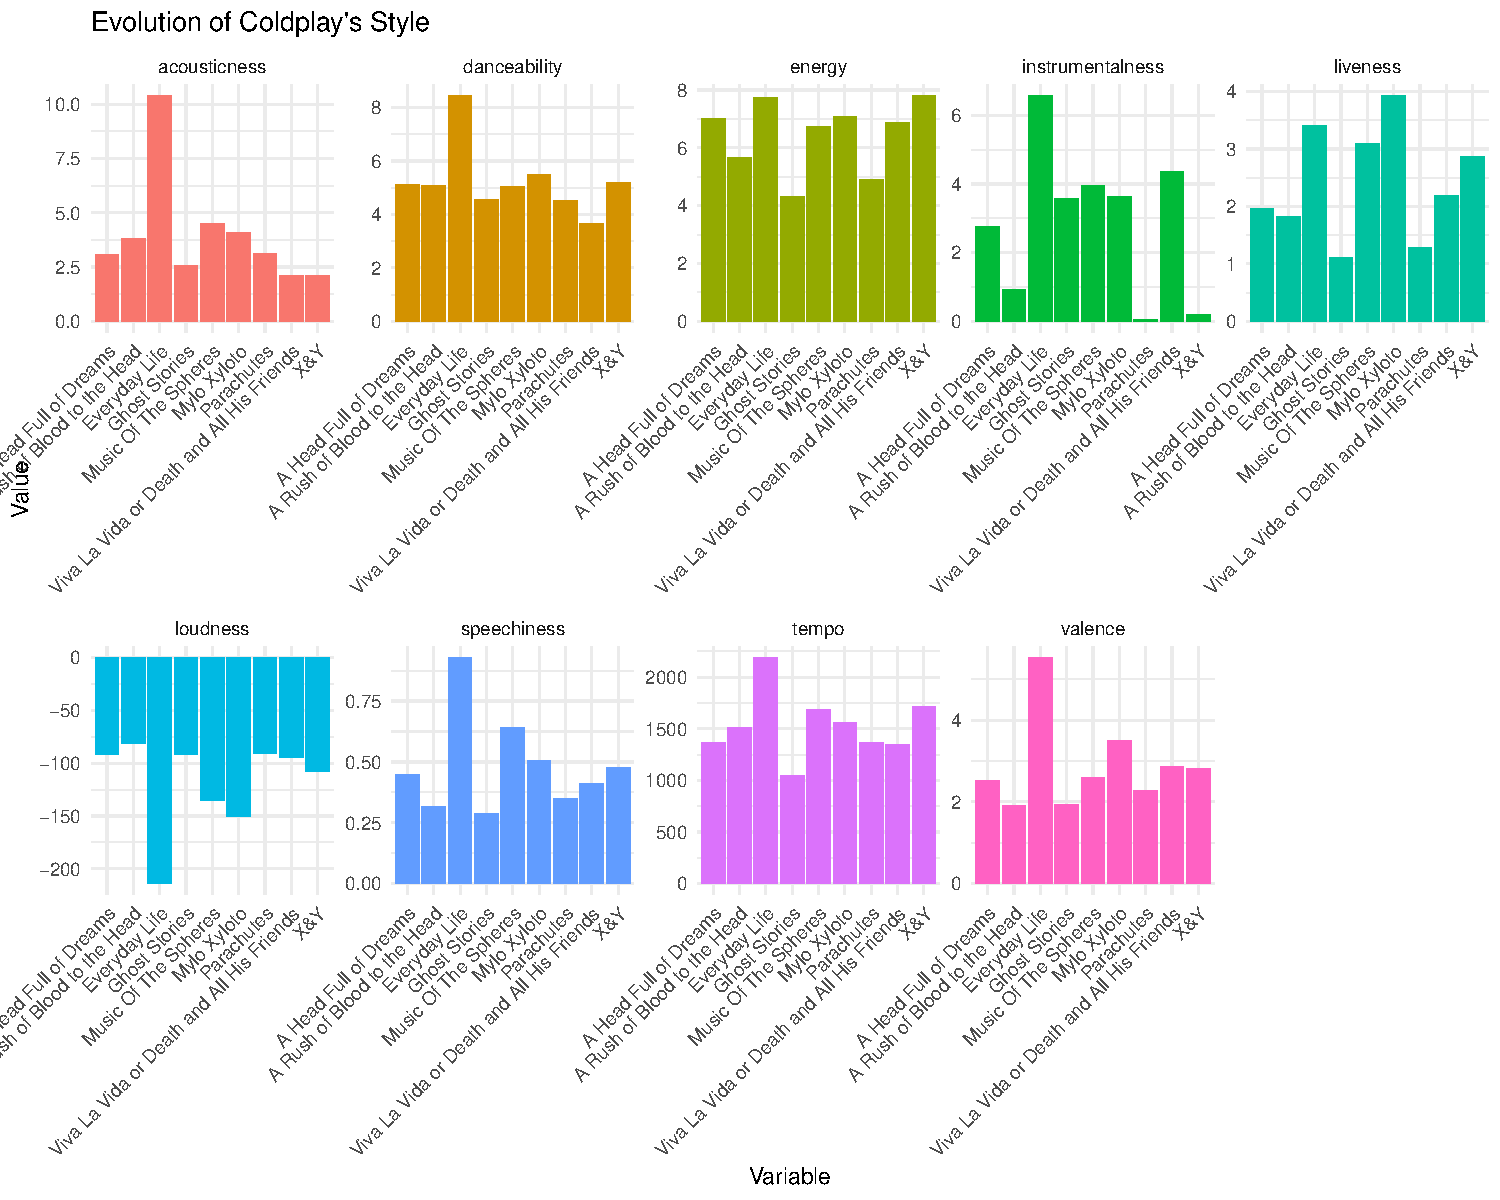
\includegraphics[angle=90]{Question3_files/figure-latex/unnamed-chunk-3-1}

Among all the albums, ``A Rush of Blood to the Head'' stands out for its
remarkable combination of acousticness, danceability, energy,
instrumentalness, liveness, loudness, speechiness, valence, and tempo.
On the other hand, the most popular album, ``Parachutes,'' does not
exhibit any distinctive characteristics that distinguish it from the
other albums.

\hypertarget{metallica-1}{%
\subsection{Metallica}\label{metallica-1}}

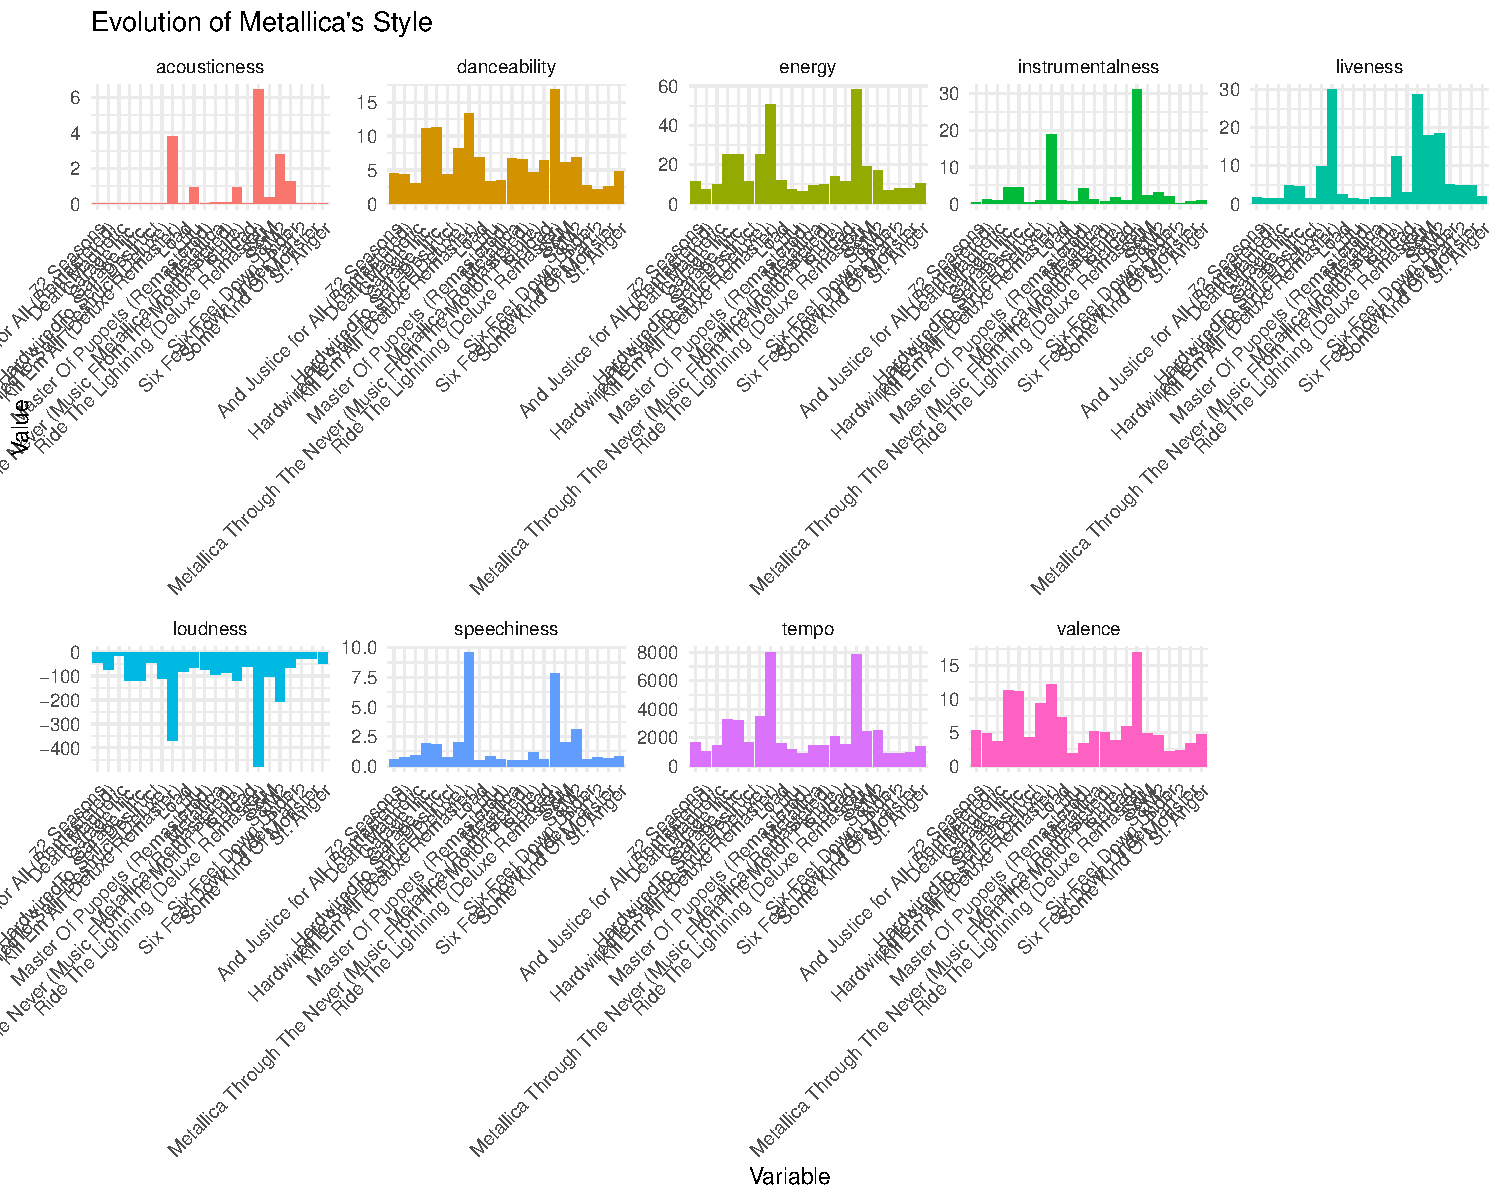
\includegraphics[angle=90]{Question3_files/figure-latex/unnamed-chunk-4-1}

In general, Metallica's albums exhibit lower levels of speechiness
compared to Coldplay. Furthermore, when it comes to danceability,
energy, instrumentalness, liveness, loudness, valence, and tempo,
Metallica's albums diverge significantly from Coldplay's, showcasing a
distinct and more pronounced range.

\hypertarget{part-c}{%
\section{Part C}\label{part-c}}

In this section, I explore the emotional characteristics of each album,
focusing on two primary emotions: ``Happy'' and ``Sad''. To simplify the
analysis, I selected specific variables such as acousticness,
danceability, energy, instrumentalness, loudness, speechiness, valence,
and tempo. I established threshold values for each variable by
referencing the emotional qualities of Coldplay's saddest and happiest
songs, leveraging my familiarity with their music.

\hypertarget{coldplay-2}{%
\subsection{Coldplay}\label{coldplay-2}}

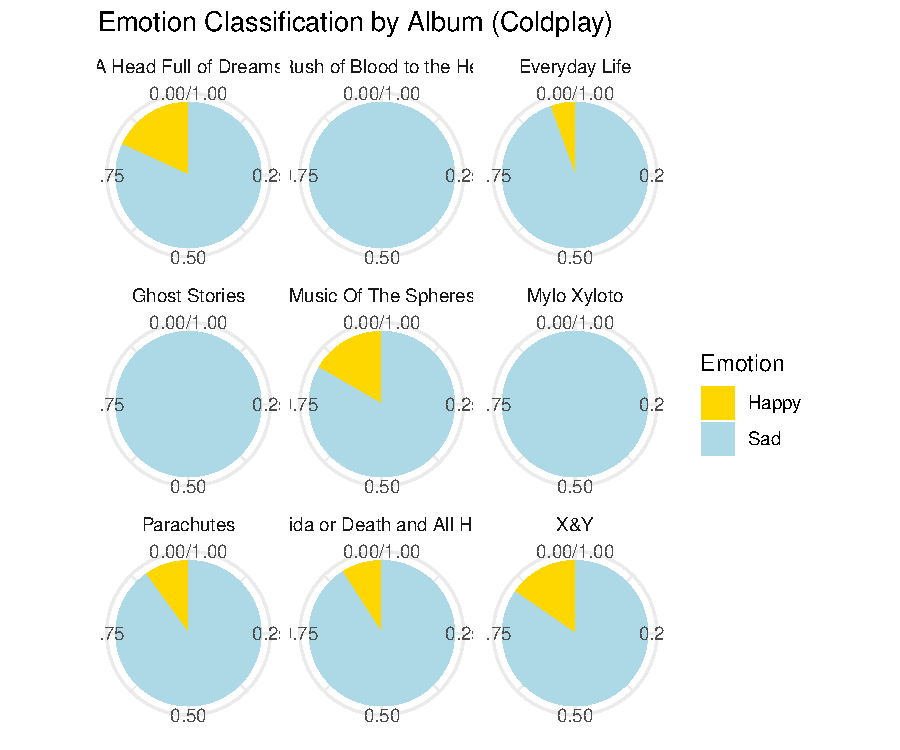
\includegraphics{Question3_files/figure-latex/unnamed-chunk-5-1.pdf}

Overall, Coldplay's albums exhibit ``Sad'' characteristics.

\hypertarget{metallica-2}{%
\section{Metallica}\label{metallica-2}}

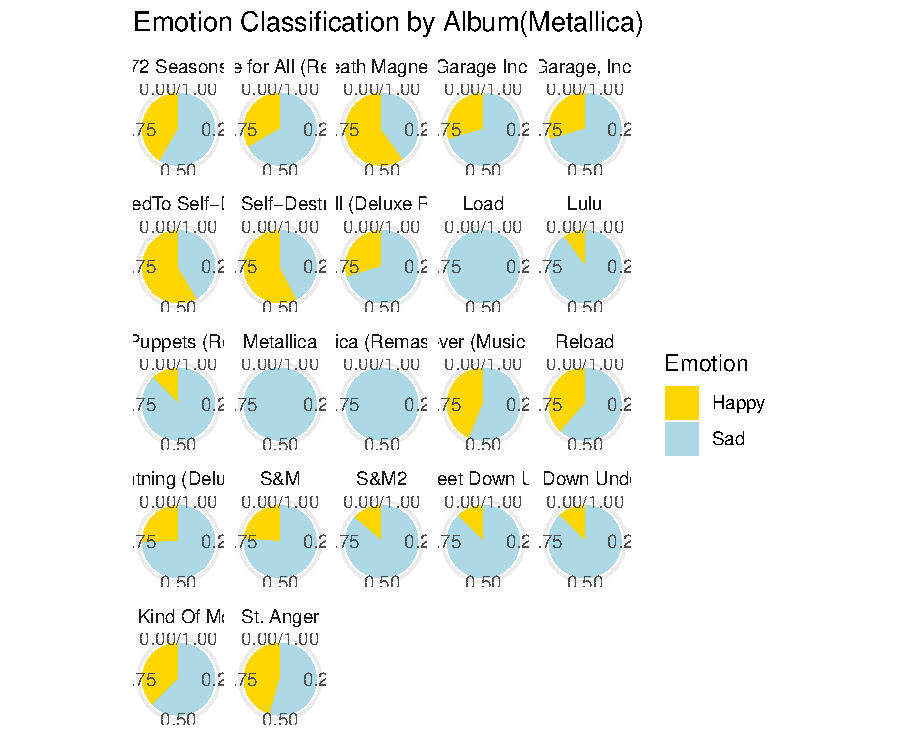
\includegraphics{Question3_files/figure-latex/unnamed-chunk-6-1.pdf}

Metallica's albums showcase a noteworthy blend of ``Happy'' and deeply
emotive compositions. While some albums lean towards a more uplifting
and energetic vibe, others delve into profound emotional depths. This
observation resonates with our earlier analysis of their style,
illuminating the multifaceted nature of Metallica's music. By exploring
both the stylistic elements and the range of emotions conveyed in their
albums, we gain a richer understanding of the artistic complexity that
defines Metallica's discography. \hfill

\hypertarget{discussion}{%
\section{Discussion}\label{discussion}}

In conclusion, by considering your desired mood, whether it be ``Happy''
or ``Sad,'' you can now select an album that perfectly aligns with your
emotional state. Coldplay's music is a poignant choice if you seek a
heartfelt catharsis, as their compositions resonate deeply and evoke
emotional responses. On the other hand, Metallica's albums offer a rich
tapestry of artistic complexity, providing a captivating journey that
demands attentive listening. However, it's worth noting that Metallica's
music is best appreciated when experienced in a deliberate sequence
rather than on shuffle mode. Regardless of your preference, both
Coldplay and Metallica offer profound musical experiences tailored to
your desired emotional landscape.

\newpage

\bibliography{Tex/ref}





\end{document}
